\KOMAoption{paper}{a4, portrait}
\areaset{267mm}{180mm}
\fancyheadoffset{0pt} % обновляем хедер и футер

\newgeometry{
  top=14mm,
  bottom=11mm,
  right=10mm,
  left=22mm,
}

\begin{landscape}

%\setlength{\headsep}{5.6mm} 
%\setlength{\topmargin}{-27mm}
\setlength{\footskip}{15.5pt}
%\setlength{\textwidth}{305mm}

\color{uniblue}{\section[(справочное) Перечень сигналов ФСУ, предназначенных для \newline конфигурирования устройства]{(справочное)\\Перечень сигналов ФСУ, предназначенных для конфигурирования устройства}\label{app:signals}}
\color{black}

\begin{enumerate}[label=\ref{app:signals}.\arabic*] % Без глобального влияния
  \item Перечень сигналов самодиагностики, доступных для конфигурирования, приведен в документации \ManualUnitGeneral.
  \item Условные обозначения, применяемые в таблице перечня сигналов:
  \begin{itemize}
    \item[$\text{(--)}$] { - сигнал не имеет возможности конфигурации;}
    \item[$\text{(+)}$] { - сигнал имеет возможность конфигурации;}
    \item[$\text{(*)}$] { - конфигурация сигнала предустановлена по умолчанию в сервисном ПО «ЮНИТ-СЕРВИС» и не может быть изменена.}
  \end{itemize}
\end{enumerate}

\small % сделаем шрифт в таблице поменьше
% В таблице ниже убрал правую и левую горизонтальные линии чтобы не сливались и жирно видно - также в настройках geometry прищлось поле right =8mm а не 5 mm 
% так как строки ниже колонтитулов спускались
\begin{longtable}{
>{\centering\arraybackslash}m{6.0cm}
|>{\centering\arraybackslash}m{3.45cm}
|>{\centering\arraybackslash}m{2cm}
|>{\centering\arraybackslash}m{2cm}
|>{\centering\arraybackslash}m{2cm}
|>{\centering\arraybackslash}m{2cm}
|>{\centering\arraybackslash}m{2cm}
|>{\centering\arraybackslash}m{2cm}
|>{\centering\arraybackslash}m{2.107cm}
}

%\caption{Перечень сигналов ФСУ, предназначенных для конфигурирования устройств ЮНИТ-М300\vspace{-0.5\baselineskip}}\label{appA:tbl1}\\ % выравнивает надпись посередине таблицы
\caption{Перечень сигналов ФСУ, предназначенных для конфигурирования устройства\hfill\vspace{-0.5\baselineskip}}\label{appA:tbl1}\\ 

\hline
\rowcolor{gray!30}
Полное наименование сигнала & Наименование сигнала на ФСУ & Дискретные входы & Выходные реле & Светодиоды & Функционал. клавиши & Регистратор событий & Аварийный осциллограф & Пуск авар. осциллографа \\ 
\hline
\endfirsthead
%\caption{\emph{Продолжение\vspace{-0.5\baselineskip}}} \\ % Отступ обозначения таблицы от таблицы и выравнивание надписи слева
\caption*{\hspace{3pt}\emph{Продолжение таблицы \ref{appA:tbl1}\hfill\vspace{-0.5\baselineskip}}} \\ % сделано по ГОСТ 2.105 п.6.8.7
\hline
\rowcolor{gray!30}
Полное наименование сигнала & Наименование сигнала на ФСУ & Дискретные входы & Выходные реле & Светодиоды & Функционал. клавиши & Регистратор событий & Аварийный осциллограф & Пуск авар. осциллографа \\ 
%\hline
\endhead

%\hline
\endfoot

%\hline
\endlastfoot

%===t2
\multicolumn{9}{c}{\textbf{Общие сигналы функциональной логики}} \\
\hline
\rowcolor{gray!15}
\multicolumn{9}{c}{ДТЗ } \\
\hline
\multicolumn{9}{c}{ Общие сигналы блока } \\
\hline
\raggedright ДТЗ: Срабатывание фА & \centering ДТЗ: Срабатывание фА & \centering -- & \centering -- & \centering -- & \centering -- & \centering -- & \centering -- & \centering \arraybackslash -- \\ \hline
\raggedright ДТЗ: Срабатывание & \centering ДТЗ: Срабатывание & \centering -- & \centering -- & \centering -- & \centering -- & \centering -- & \centering -- & \centering \arraybackslash -- \\ \hline
\raggedright ДТЗ: Срабатывание фС & \centering ДТЗ: Срабатывание фС & \centering -- & \centering -- & \centering -- & \centering -- & \centering -- & \centering -- & \centering \arraybackslash -- \\ \hline
\raggedright ДТЗ: Срабатывание фВ & \centering ДТЗ: Срабатывание фВ & \centering -- & \centering -- & \centering -- & \centering -- & \centering -- & \centering -- & \centering \arraybackslash -- \\ \hline
\multicolumn{9}{c}{\text{Д2г}} \\
\hline
\raggedright ДТЗ/ Д2г: Срабатывание фA & \centering ДТЗ/ Д2г: Срабатывание фA & \centering -- & \centering -- & \centering -- & \centering -- & \centering -- & \centering -- & \centering \arraybackslash -- \\ \hline
\raggedright ДТЗ/ Д2г: Срабатывание фB & \centering ДТЗ/ Д2г: Срабатывание фB & \centering -- & \centering -- & \centering -- & \centering -- & \centering -- & \centering -- & \centering \arraybackslash -- \\ \hline
\raggedright ДТЗ/ Д2г: Срабатывание фC & \centering ДТЗ/ Д2г: Срабатывание фC & \centering -- & \centering -- & \centering -- & \centering -- & \centering -- & \centering -- & \centering \arraybackslash -- \\ \hline
\raggedright ДТЗ/ Д2г: Выведено & \centering ДТЗ/ Д2г: Выведено & \centering -- & \centering -- & \centering -- & \centering -- & \centering -- & \centering -- & \centering \arraybackslash -- \\ \hline
\multicolumn{9}{c}{\text{Д5г}} \\
\hline
\raggedright ДТЗ/ Д5г: Срабатывание фA & \centering ДТЗ/ Д5г: Срабатывание фA & \centering -- & \centering -- & \centering -- & \centering -- & \centering -- & \centering -- & \centering \arraybackslash -- \\ \hline
\raggedright ДТЗ/ Д5г: Срабатывание фB & \centering ДТЗ/ Д5г: Срабатывание фB & \centering -- & \centering -- & \centering -- & \centering -- & \centering -- & \centering -- & \centering \arraybackslash -- \\ \hline
\raggedright ДТЗ/ Д5г: Срабатывание фC & \centering ДТЗ/ Д5г: Срабатывание фC & \centering -- & \centering -- & \centering -- & \centering -- & \centering -- & \centering -- & \centering \arraybackslash -- \\ \hline
\raggedright ДТЗ/ Д5г: Выведено & \centering ДТЗ/ Д5г: Выведено & \centering -- & \centering -- & \centering -- & \centering -- & \centering -- & \centering -- & \centering \arraybackslash -- \\ \hline
\multicolumn{9}{c}{\text{ДТЗт}} \\
\hline
\raggedright ДТЗ/ ДТЗт: ИО фА & \centering ДТЗ/ ДТЗт: ИО фА & \centering -- & \centering -- & \centering -- & \centering -- & \centering -- & \centering -- & \centering \arraybackslash -- \\ \hline
\raggedright ДТЗ/ ДТЗт: Срабатывание фА & \centering ДТЗ/ ДТЗт: Срабатывание фА & \centering -- & \centering -- & \centering -- & \centering -- & \centering -- & \centering -- & \centering \arraybackslash -- \\ \hline
\raggedright ДТЗ/ ДТЗт: Срабатывание фB & \centering ДТЗ/ ДТЗт: Срабатывание фB & \centering -- & \centering -- & \centering -- & \centering -- & \centering -- & \centering -- & \centering \arraybackslash -- \\ \hline
\raggedright ДТЗ/ ДТЗт: ИО фB & \centering ДТЗ/ ДТЗт: ИО фB & \centering -- & \centering -- & \centering -- & \centering -- & \centering -- & \centering -- & \centering \arraybackslash -- \\ \hline
\raggedright ДТЗ/ ДТЗт: ИО фC & \centering ДТЗ/ ДТЗт: ИО фC & \centering -- & \centering -- & \centering -- & \centering -- & \centering -- & \centering -- & \centering \arraybackslash -- \\ \hline
\raggedright ДТЗ/ ДТЗт: Срабатывание фC & \centering ДТЗ/ ДТЗт: Срабатывание фC & \centering -- & \centering -- & \centering -- & \centering -- & \centering -- & \centering -- & \centering \arraybackslash -- \\ \hline
\raggedright ДТЗ/ ДТЗт: Выведено & \centering ДТЗ/ ДТЗт: Выведено & \centering -- & \centering -- & \centering -- & \centering -- & \centering -- & \centering -- & \centering \arraybackslash -- \\ \hline
\multicolumn{9}{c}{\text{ДТО}} \\
\hline
\raggedright ДТЗ/ ДТО: ИО фА & \centering ДТЗ/ ДТО: ИО фА & \centering -- & \centering -- & \centering -- & \centering -- & \centering -- & \centering -- & \centering \arraybackslash -- \\ \hline
\raggedright ДТЗ/ ДТО: Срабатывание фА & \centering ДТЗ/ ДТО: Срабатывание фА & \centering -- & \centering -- & \centering -- & \centering -- & \centering -- & \centering -- & \centering \arraybackslash -- \\ \hline
\raggedright ДТЗ/ ДТО: ИО фB & \centering ДТЗ/ ДТО: ИО фB & \centering -- & \centering -- & \centering -- & \centering -- & \centering -- & \centering -- & \centering \arraybackslash -- \\ \hline
\raggedright ДТЗ/ ДТО: ИО фC & \centering ДТЗ/ ДТО: ИО фC & \centering -- & \centering -- & \centering -- & \centering -- & \centering -- & \centering -- & \centering \arraybackslash -- \\ \hline
\raggedright ДТЗ/ ДТО: Срабатывание фB & \centering ДТЗ/ ДТО: Срабатывание фB & \centering -- & \centering -- & \centering -- & \centering -- & \centering -- & \centering -- & \centering \arraybackslash -- \\ \hline
\raggedright ДТЗ/ ДТО: Срабатывание фC & \centering ДТЗ/ ДТО: Срабатывание фC & \centering -- & \centering -- & \centering -- & \centering -- & \centering -- & \centering -- & \centering \arraybackslash -- \\ \hline
\raggedright ДТЗ/ ДТО: Выведено & \centering ДТЗ/ ДТО: Выведено & \centering -- & \centering -- & \centering -- & \centering -- & \centering -- & \centering -- & \centering \arraybackslash -- \\ \hline
\multicolumn{9}{c}{\text{КЦТ}} \\
\hline
\raggedright ДТЗ/ КЦТ: Срабатывание & \centering ДТЗ/ КЦТ: Срабатывание & \centering -- & \centering -- & \centering -- & \centering -- & \centering -- & \centering -- & \centering \arraybackslash -- \\ \hline
\rowcolor{gray!15}
\multicolumn{9}{c}{КИ НН } \\
\hline
\multicolumn{9}{c}{\text{ИО КН}} \\
\hline
\raggedright КИ НН/ ИО КН: Пуск & \centering КИ НН/ ИО КН: Пуск & \centering -- & \centering -- & \centering -- & \centering -- & \centering -- & \centering -- & \centering \arraybackslash -- \\ \hline
\raggedright КИ НН/ ИО КН: Срабатывание & \centering КИ НН/ ИО КН: Срабатывание & \centering -- & \centering -- & \centering -- & \centering -- & \centering -- & \centering -- & \centering \arraybackslash -- \\ \hline
\raggedright КИ НН/ ИО КН: Выведено & \centering КИ НН/ ИО КН: Выведено & \centering -- & \centering -- & \centering -- & \centering -- & \centering -- & \centering -- & \centering \arraybackslash -- \\ \hline
\rowcolor{gray!15}
\multicolumn{9}{c}{ЛО В1 ВН } \\
\hline
\multicolumn{9}{c}{\text{ЛО В УШР}} \\
\hline
\raggedright ЛО В1 ВН/ ЛО В УШР: Отключение & \centering ЛО В1 ВН/ ЛО В УШР: Отключение & \centering -- & \centering -- & \centering -- & \centering -- & \centering -- & \centering -- & \centering \arraybackslash -- \\ \hline
\raggedright ЛО В1 ВН/ ЛО В УШР: Выведено & \centering ЛО В1 ВН/ ЛО В УШР: Выведено & \centering -- & \centering -- & \centering -- & \centering -- & \centering -- & \centering -- & \centering \arraybackslash -- \\ \hline
\raggedright ЛО В1 ВН/ ЛО В УШР: Запрет АПВ & \centering ЛО В1 ВН/ ЛО В УШР: Запрет АПВ & \centering -- & \centering -- & \centering -- & \centering -- & \centering -- & \centering -- & \centering \arraybackslash -- \\ \hline
\rowcolor{gray!15}
\multicolumn{9}{c}{ЛО В2 ВН } \\
\hline
\multicolumn{9}{c}{\text{ЛО В УШР}} \\
\hline
\raggedright ЛО В2 ВН/ ЛО В УШР: Отключение & \centering ЛО В2 ВН/ ЛО В УШР: Отключение & \centering -- & \centering -- & \centering -- & \centering -- & \centering -- & \centering -- & \centering \arraybackslash -- \\ \hline
\raggedright ЛО В2 ВН/ ЛО В УШР: Выведено & \centering ЛО В2 ВН/ ЛО В УШР: Выведено & \centering -- & \centering -- & \centering -- & \centering -- & \centering -- & \centering -- & \centering \arraybackslash -- \\ \hline
\raggedright ЛО В2 ВН/ ЛО В УШР: Запрет АПВ & \centering ЛО В2 ВН/ ЛО В УШР: Запрет АПВ & \centering -- & \centering -- & \centering -- & \centering -- & \centering -- & \centering -- & \centering \arraybackslash -- \\ \hline
\rowcolor{gray!15}
\multicolumn{9}{c}{ЛО ТМПд } \\
\hline
\multicolumn{9}{c}{\text{ЛО В УШР}} \\
\hline
\raggedright ЛО ТМПд/ ЛО В УШР: Отключение & \centering ЛО ТМПд/ ЛО В УШР: Отключение & \centering -- & \centering -- & \centering -- & \centering -- & \centering -- & \centering -- & \centering \arraybackslash -- \\ \hline
\raggedright ЛО ТМПд/ ЛО В УШР: Выведено & \centering ЛО ТМПд/ ЛО В УШР: Выведено & \centering -- & \centering -- & \centering -- & \centering -- & \centering -- & \centering -- & \centering \arraybackslash -- \\ \hline
\raggedright ЛО ТМПд/ ЛО В УШР: Запрет АПВ & \centering ЛО ТМПд/ ЛО В УШР: Запрет АПВ & \centering -- & \centering -- & \centering -- & \centering -- & \centering -- & \centering -- & \centering \arraybackslash -- \\ \hline
\rowcolor{gray!15}
\multicolumn{9}{c}{ЛО ТМПо } \\
\hline
\multicolumn{9}{c}{\text{ЛО В УШР}} \\
\hline
\raggedright ЛО ТМПо/ ЛО В УШР: Отключение & \centering ЛО ТМПо/ ЛО В УШР: Отключение & \centering -- & \centering -- & \centering -- & \centering -- & \centering -- & \centering -- & \centering \arraybackslash -- \\ \hline
\raggedright ЛО ТМПо/ ЛО В УШР: Выведено & \centering ЛО ТМПо/ ЛО В УШР: Выведено & \centering -- & \centering -- & \centering -- & \centering -- & \centering -- & \centering -- & \centering \arraybackslash -- \\ \hline
\raggedright ЛО ТМПо/ ЛО В УШР: Запрет АПВ & \centering ЛО ТМПо/ ЛО В УШР: Запрет АПВ & \centering -- & \centering -- & \centering -- & \centering -- & \centering -- & \centering -- & \centering \arraybackslash -- \\ \hline
\rowcolor{gray!15}
\multicolumn{9}{c}{ЛО ТМПр } \\
\hline
\multicolumn{9}{c}{\text{ЛО В УШР}} \\
\hline
\raggedright ЛО ТМПр/ ЛО В УШР: Отключение & \centering ЛО ТМПр/ ЛО В УШР: Отключение & \centering -- & \centering -- & \centering -- & \centering -- & \centering -- & \centering -- & \centering \arraybackslash -- \\ \hline
\raggedright ЛО ТМПр/ ЛО В УШР: Выведено & \centering ЛО ТМПр/ ЛО В УШР: Выведено & \centering -- & \centering -- & \centering -- & \centering -- & \centering -- & \centering -- & \centering \arraybackslash -- \\ \hline
\raggedright ЛО ТМПр/ ЛО В УШР: Запрет АПВ & \centering ЛО ТМПр/ ЛО В УШР: Запрет АПВ & \centering -- & \centering -- & \centering -- & \centering -- & \centering -- & \centering -- & \centering \arraybackslash -- \\ \hline
\rowcolor{gray!15}
\multicolumn{9}{c}{МТЗ КО } \\
\hline
\multicolumn{9}{c}{ Общие сигналы блока } \\
\hline
\raggedright МТЗ КО: Пуск & \centering МТЗ КО: Пуск & \centering -- & \centering -- & \centering -- & \centering -- & \centering -- & \centering -- & \centering \arraybackslash -- \\ \hline
\raggedright МТЗ КО: Срабатывание & \centering МТЗ КО: Срабатывание & \centering -- & \centering -- & \centering -- & \centering -- & \centering -- & \centering -- & \centering \arraybackslash -- \\ \hline
\multicolumn{9}{c}{\text{МТЗ КО-1}} \\
\hline
\raggedright МТЗ КО/ МТЗ КО-1: ИО МТЗ & \centering МТЗ КО/ МТЗ КО-1: ИО МТЗ & \centering -- & \centering -- & \centering -- & \centering -- & \centering -- & \centering -- & \centering \arraybackslash -- \\ \hline
\raggedright МТЗ КО/ МТЗ КО-1: Пуск & \centering МТЗ КО/ МТЗ КО-1: Пуск & \centering -- & \centering -- & \centering -- & \centering -- & \centering -- & \centering -- & \centering \arraybackslash -- \\ \hline
\raggedright МТЗ КО/ МТЗ КО-1: Срабатывание & \centering МТЗ КО/ МТЗ КО-1: Срабатывание & \centering -- & \centering -- & \centering -- & \centering -- & \centering -- & \centering -- & \centering \arraybackslash -- \\ \hline
\raggedright МТЗ КО/ МТЗ КО-1: Выведено & \centering МТЗ КО/ МТЗ КО-1: Выведено & \centering -- & \centering -- & \centering -- & \centering -- & \centering -- & \centering -- & \centering \arraybackslash -- \\ \hline
\multicolumn{9}{c}{\text{МТЗ КО-2}} \\
\hline
\raggedright МТЗ КО/ МТЗ КО-2: ИО МТЗ & \centering МТЗ КО/ МТЗ КО-2: ИО МТЗ & \centering -- & \centering -- & \centering -- & \centering -- & \centering -- & \centering -- & \centering \arraybackslash -- \\ \hline
\raggedright МТЗ КО/ МТЗ КО-2: Пуск & \centering МТЗ КО/ МТЗ КО-2: Пуск & \centering -- & \centering -- & \centering -- & \centering -- & \centering -- & \centering -- & \centering \arraybackslash -- \\ \hline
\raggedright МТЗ КО/ МТЗ КО-2: Срабатывание & \centering МТЗ КО/ МТЗ КО-2: Срабатывание & \centering -- & \centering -- & \centering -- & \centering -- & \centering -- & \centering -- & \centering \arraybackslash -- \\ \hline
\raggedright МТЗ КО/ МТЗ КО-2: Выведено & \centering МТЗ КО/ МТЗ КО-2: Выведено & \centering -- & \centering -- & \centering -- & \centering -- & \centering -- & \centering -- & \centering \arraybackslash -- \\ \hline
\rowcolor{gray!15}
\multicolumn{9}{c}{МТЗ НН } \\
\hline
\multicolumn{9}{c}{ Общие сигналы блока } \\
\hline
\raggedright МТЗ НН: Пуск & \centering МТЗ НН: Пуск & \centering -- & \centering -- & \centering -- & \centering -- & \centering -- & \centering -- & \centering \arraybackslash -- \\ \hline
\raggedright МТЗ НН: Србатывание & \centering МТЗ НН: Србатывание & \centering -- & \centering -- & \centering -- & \centering -- & \centering -- & \centering -- & \centering \arraybackslash -- \\ \hline
\multicolumn{9}{c}{\text{МТЗ-1}} \\
\hline
\raggedright МТЗ НН/ МТЗ-1: ИО МТЗ & \centering МТЗ НН/ МТЗ-1: ИО МТЗ & \centering -- & \centering -- & \centering -- & \centering -- & \centering -- & \centering -- & \centering \arraybackslash -- \\ \hline
\raggedright МТЗ НН/ МТЗ-1: Пуск & \centering МТЗ НН/ МТЗ-1: Пуск & \centering -- & \centering -- & \centering -- & \centering -- & \centering -- & \centering -- & \centering \arraybackslash -- \\ \hline
\raggedright МТЗ НН/ МТЗ-1: Срабатывание & \centering МТЗ НН/ МТЗ-1: Срабатывание & \centering -- & \centering -- & \centering -- & \centering -- & \centering -- & \centering -- & \centering \arraybackslash -- \\ \hline
\raggedright МТЗ НН/ МТЗ-1: Выведено & \centering МТЗ НН/ МТЗ-1: Выведено & \centering -- & \centering -- & \centering -- & \centering -- & \centering -- & \centering -- & \centering \arraybackslash -- \\ \hline
\multicolumn{9}{c}{\text{МТЗ-2}} \\
\hline
\raggedright МТЗ НН/ МТЗ-2: ИО МТЗ & \centering МТЗ НН/ МТЗ-2: ИО МТЗ & \centering -- & \centering -- & \centering -- & \centering -- & \centering -- & \centering -- & \centering \arraybackslash -- \\ \hline
\raggedright МТЗ НН/ МТЗ-2: Пуск & \centering МТЗ НН/ МТЗ-2: Пуск & \centering -- & \centering -- & \centering -- & \centering -- & \centering -- & \centering -- & \centering \arraybackslash -- \\ \hline
\raggedright МТЗ НН/ МТЗ-2: Срабатывание & \centering МТЗ НН/ МТЗ-2: Срабатывание & \centering -- & \centering -- & \centering -- & \centering -- & \centering -- & \centering -- & \centering \arraybackslash -- \\ \hline
\raggedright МТЗ НН/ МТЗ-2: Выведено & \centering МТЗ НН/ МТЗ-2: Выведено & \centering -- & \centering -- & \centering -- & \centering -- & \centering -- & \centering -- & \centering \arraybackslash -- \\ \hline
\rowcolor{gray!15}
\multicolumn{9}{c}{МТЗ ОУ } \\
\hline
\multicolumn{9}{c}{\text{МТЗ ОУ}} \\
\hline
\raggedright МТЗ ОУ/ МТЗ ОУ: Выведено & \centering МТЗ ОУ/ МТЗ ОУ: Выведено & \centering -- & \centering -- & \centering -- & \centering -- & \centering -- & \centering -- & \centering \arraybackslash -- \\ \hline
\raggedright МТЗ ОУ/ МТЗ ОУ: Срабатывание & \centering МТЗ ОУ/ МТЗ ОУ: Срабатывание & \centering -- & \centering -- & \centering -- & \centering -- & \centering -- & \centering -- & \centering \arraybackslash -- \\ \hline
\raggedright МТЗ ОУ/ МТЗ ОУ: Пуск & \centering МТЗ ОУ/ МТЗ ОУ: Пуск & \centering -- & \centering -- & \centering -- & \centering -- & \centering -- & \centering -- & \centering \arraybackslash -- \\ \hline
\raggedright МТЗ ОУ/ МТЗ ОУ: ИО МТЗ & \centering МТЗ ОУ/ МТЗ ОУ: ИО МТЗ & \centering -- & \centering -- & \centering -- & \centering -- & \centering -- & \centering -- & \centering \arraybackslash -- \\ \hline
\rowcolor{gray!15}
\multicolumn{9}{c}{ОВ БНТ ВВ } \\
\hline
\multicolumn{9}{c}{\text{ОВ БНТ}} \\
\hline
\raggedright ОВ БНТ ВВ/ ОВ БНТ: Выведено & \centering ОВ БНТ ВВ/ ОВ БНТ: Выведено & \centering -- & \centering -- & \centering -- & \centering -- & \centering -- & \centering -- & \centering \arraybackslash -- \\ \hline
\raggedright ОВ БНТ ВВ/ ОВ БНТ: Срабатывание & \centering ОВ БНТ ВВ/ ОВ БНТ: Срабатывание & \centering -- & \centering -- & \centering -- & \centering -- & \centering -- & \centering -- & \centering \arraybackslash -- \\ \hline
\raggedright ОВ БНТ ВВ/ ОВ БНТ: Срабатывание фC(CA) & \centering ОВ БНТ ВВ/ ОВ БНТ: Срабатывание фC(CA) & \centering -- & \centering -- & \centering -- & \centering -- & \centering -- & \centering -- & \centering \arraybackslash -- \\ \hline
\raggedright ОВ БНТ ВВ/ ОВ БНТ: Срабатывание фB(BC) & \centering ОВ БНТ ВВ/ ОВ БНТ: Срабатывание фB(BC) & \centering -- & \centering -- & \centering -- & \centering -- & \centering -- & \centering -- & \centering \arraybackslash -- \\ \hline
\raggedright ОВ БНТ ВВ/ ОВ БНТ: Срабатывание фA(AB) & \centering ОВ БНТ ВВ/ ОВ БНТ: Срабатывание фA(AB) & \centering -- & \centering -- & \centering -- & \centering -- & \centering -- & \centering -- & \centering \arraybackslash -- \\ \hline
\rowcolor{gray!15}
\multicolumn{9}{c}{Общая ЛО УШР } \\
\hline
\multicolumn{9}{c}{\text{ЛО ОЗ}} \\
\hline
\raggedright Общая ЛО УШР/ ЛО ОЗ: Срабатывание & \centering Общая ЛО УШР/ ЛО ОЗ: Срабатывание & \centering -- & \centering -- & \centering -- & \centering -- & \centering -- & \centering -- & \centering \arraybackslash -- \\ \hline
\multicolumn{9}{c}{\text{ЛО РЗ}} \\
\hline
\raggedright Общая ЛО УШР/ ЛО РЗ: Срабатывание & \centering Общая ЛО УШР/ ЛО РЗ: Срабатывание & \centering -- & \centering -- & \centering -- & \centering -- & \centering -- & \centering -- & \centering \arraybackslash -- \\ \hline
\multicolumn{9}{c}{\text{ЛО внеш. З}} \\
\hline
\raggedright Общая ЛО УШР/ ЛО внеш. З: Срабатывание & \centering Общая ЛО УШР/ ЛО внеш. З: Срабатывание & \centering -- & \centering -- & \centering -- & \centering -- & \centering -- & \centering -- & \centering \arraybackslash -- \\ \hline
\rowcolor{gray!15}
\multicolumn{9}{c}{Общая логика } \\
\hline
\multicolumn{9}{c}{ Общие сигналы блока } \\
\hline
\raggedright Общая логика: БИ выведены & \centering Общая логика: БИ выведены & \centering -- & \centering -- & \centering -- & \centering -- & \centering -- & \centering -- & \centering \arraybackslash -- \\ \hline
\raggedright Общая логика: Неиспр. ОТ ЗДЗ НН & \centering Общая логика: Неиспр. ОТ ЗДЗ НН & \centering -- & \centering -- & \centering -- & \centering -- & \centering -- & \centering -- & \centering \arraybackslash -- \\ \hline
\raggedright Общая логика: Вых. цепи разобраны & \centering Общая логика: Вых. цепи разобраны & \centering -- & \centering -- & \centering -- & \centering -- & \centering -- & \centering -- & \centering \arraybackslash -- \\ \hline
\raggedright Общая логика: Неиспр. ОТ ТМПо & \centering Общая логика: Неиспр. ОТ ТМПо & \centering -- & \centering -- & \centering -- & \centering -- & \centering -- & \centering -- & \centering \arraybackslash -- \\ \hline
\raggedright Общая логика: Неиспр. ОТ & \centering Общая логика: Неиспр. ОТ & \centering -- & \centering -- & \centering -- & \centering -- & \centering -- & \centering -- & \centering \arraybackslash -- \\ \hline
\raggedright Общая логика: Неиспр. ОТ ТМПр & \centering Общая логика: Неиспр. ОТ ТМПр & \centering -- & \centering -- & \centering -- & \centering -- & \centering -- & \centering -- & \centering \arraybackslash -- \\ \hline
\rowcolor{gray!15}
\multicolumn{9}{c}{Сигнализация } \\
\hline
\multicolumn{9}{c}{ Общие сигналы блока } \\
\hline
\raggedright Сигнализация: Неиспр. ОТ & \centering Сигнализация: Неиспр. ОТ & \centering -- & \centering -- & \centering -- & \centering -- & \centering -- & \centering -- & \centering \arraybackslash -- \\ \hline
\raggedright Сигнализация: Срабатывание фикс & \centering Сигнализация: Срабатывание фикс & \centering -- & \centering -- & \centering -- & \centering -- & \centering -- & \centering -- & \centering \arraybackslash -- \\ \hline
\raggedright Сигнализация: Срабатывание имп & \centering Сигнализация: Срабатывание имп & \centering -- & \centering -- & \centering -- & \centering -- & \centering -- & \centering -- & \centering \arraybackslash -- \\ \hline
\raggedright Сигнализация: Пред. сигнализация & \centering Сигнализация: Пред. сигнализация & \centering -- & \centering -- & \centering -- & \centering -- & \centering -- & \centering -- & \centering \arraybackslash -- \\ \hline
\raggedright Сигнализация: Сигнализация фикс & \centering Сигнализация: Сигнализация фикс & \centering -- & \centering -- & \centering -- & \centering -- & \centering -- & \centering -- & \centering \arraybackslash -- \\ \hline
\raggedright Сигнализация: Сигнализация имп & \centering Сигнализация: Сигнализация имп & \centering -- & \centering -- & \centering -- & \centering -- & \centering -- & \centering -- & \centering \arraybackslash -- \\ \hline
\rowcolor{gray!15}
\multicolumn{9}{c}{ТЗНП КО } \\
\hline
\multicolumn{9}{c}{ Общие сигналы блока } \\
\hline
\raggedright ТЗНП КО: Пуск & \centering ТЗНП КО: Пуск & \centering -- & \centering -- & \centering -- & \centering -- & \centering -- & \centering -- & \centering \arraybackslash -- \\ \hline
\raggedright ТЗНП КО: Срабатывание & \centering ТЗНП КО: Срабатывание & \centering -- & \centering -- & \centering -- & \centering -- & \centering -- & \centering -- & \centering \arraybackslash -- \\ \hline
\multicolumn{9}{c}{\text{ТЗНП КО-1}} \\
\hline
\raggedright ТЗНП КО/ ТЗНП КО-1: ИО & \centering ТЗНП КО/ ТЗНП КО-1: ИО & \centering -- & \centering -- & \centering -- & \centering -- & \centering -- & \centering -- & \centering \arraybackslash -- \\ \hline
\raggedright ТЗНП КО/ ТЗНП КО-1: Выведено & \centering ТЗНП КО/ ТЗНП КО-1: Выведено & \centering -- & \centering -- & \centering -- & \centering -- & \centering -- & \centering -- & \centering \arraybackslash -- \\ \hline
\raggedright ТЗНП КО/ ТЗНП КО-1: Срабатывание & \centering ТЗНП КО/ ТЗНП КО-1: Срабатывание & \centering -- & \centering -- & \centering -- & \centering -- & \centering -- & \centering -- & \centering \arraybackslash -- \\ \hline
\raggedright ТЗНП КО/ ТЗНП КО-1: Пуск & \centering ТЗНП КО/ ТЗНП КО-1: Пуск & \centering -- & \centering -- & \centering -- & \centering -- & \centering -- & \centering -- & \centering \arraybackslash -- \\ \hline
\multicolumn{9}{c}{\text{ТЗНП КО-2}} \\
\hline
\raggedright ТЗНП КО/ ТЗНП КО-2: ИО & \centering ТЗНП КО/ ТЗНП КО-2: ИО & \centering -- & \centering -- & \centering -- & \centering -- & \centering -- & \centering -- & \centering \arraybackslash -- \\ \hline
\raggedright ТЗНП КО/ ТЗНП КО-2: Выведено & \centering ТЗНП КО/ ТЗНП КО-2: Выведено & \centering -- & \centering -- & \centering -- & \centering -- & \centering -- & \centering -- & \centering \arraybackslash -- \\ \hline
\raggedright ТЗНП КО/ ТЗНП КО-2: Срабатывание & \centering ТЗНП КО/ ТЗНП КО-2: Срабатывание & \centering -- & \centering -- & \centering -- & \centering -- & \centering -- & \centering -- & \centering \arraybackslash -- \\ \hline
\raggedright ТЗНП КО/ ТЗНП КО-2: Пуск & \centering ТЗНП КО/ ТЗНП КО-2: Пуск & \centering -- & \centering -- & \centering -- & \centering -- & \centering -- & \centering -- & \centering \arraybackslash -- \\ \hline
\rowcolor{gray!15}
\multicolumn{9}{c}{ТЗОП КО } \\
\hline
\multicolumn{9}{c}{ Общие сигналы блока } \\
\hline
\raggedright ТЗОП КО: Пуск & \centering ТЗОП КО: Пуск & \centering -- & \centering -- & \centering -- & \centering -- & \centering -- & \centering -- & \centering \arraybackslash -- \\ \hline
\raggedright ТЗОП КО: Срабатывание & \centering ТЗОП КО: Срабатывание & \centering -- & \centering -- & \centering -- & \centering -- & \centering -- & \centering -- & \centering \arraybackslash -- \\ \hline
\multicolumn{9}{c}{\text{ТЗОП КО-1}} \\
\hline
\raggedright ТЗОП КО/ ТЗОП КО-1: ИО & \centering ТЗОП КО/ ТЗОП КО-1: ИО & \centering -- & \centering -- & \centering -- & \centering -- & \centering -- & \centering -- & \centering \arraybackslash -- \\ \hline
\raggedright ТЗОП КО/ ТЗОП КО-1: Выведено & \centering ТЗОП КО/ ТЗОП КО-1: Выведено & \centering -- & \centering -- & \centering -- & \centering -- & \centering -- & \centering -- & \centering \arraybackslash -- \\ \hline
\raggedright ТЗОП КО/ ТЗОП КО-1: Срабатывание & \centering ТЗОП КО/ ТЗОП КО-1: Срабатывание & \centering -- & \centering -- & \centering -- & \centering -- & \centering -- & \centering -- & \centering \arraybackslash -- \\ \hline
\raggedright ТЗОП КО/ ТЗОП КО-1: Пуск & \centering ТЗОП КО/ ТЗОП КО-1: Пуск & \centering -- & \centering -- & \centering -- & \centering -- & \centering -- & \centering -- & \centering \arraybackslash -- \\ \hline
\multicolumn{9}{c}{\text{ТЗОП КО-2}} \\
\hline
\raggedright ТЗОП КО/ ТЗОП КО-2: ИО & \centering ТЗОП КО/ ТЗОП КО-2: ИО & \centering -- & \centering -- & \centering -- & \centering -- & \centering -- & \centering -- & \centering \arraybackslash -- \\ \hline
\raggedright ТЗОП КО/ ТЗОП КО-2: Выведено & \centering ТЗОП КО/ ТЗОП КО-2: Выведено & \centering -- & \centering -- & \centering -- & \centering -- & \centering -- & \centering -- & \centering \arraybackslash -- \\ \hline
\raggedright ТЗОП КО/ ТЗОП КО-2: Срабатывание & \centering ТЗОП КО/ ТЗОП КО-2: Срабатывание & \centering -- & \centering -- & \centering -- & \centering -- & \centering -- & \centering -- & \centering \arraybackslash -- \\ \hline
\raggedright ТЗОП КО/ ТЗОП КО-2: Пуск & \centering ТЗОП КО/ ТЗОП КО-2: Пуск & \centering -- & \centering -- & \centering -- & \centering -- & \centering -- & \centering -- & \centering \arraybackslash -- \\ \hline
\rowcolor{gray!15}
\multicolumn{9}{c}{ТК ЗДЗ УШР } \\
\hline
\multicolumn{9}{c}{ Общие сигналы блока } \\
\hline
\raggedright ТК ЗДЗ УШР: Пуск & \centering ТК ЗДЗ УШР: Пуск & \centering -- & \centering -- & \centering -- & \centering -- & \centering -- & \centering -- & \centering \arraybackslash -- \\ \hline
\multicolumn{9}{c}{\text{ТК ЗДЗ КО}} \\
\hline
\raggedright ТК ЗДЗ УШР/ ТК ЗДЗ КО: Выведено & \centering ТК ЗДЗ УШР/ ТК ЗДЗ КО: Выведено & \centering -- & \centering -- & \centering -- & \centering -- & \centering -- & \centering -- & \centering \arraybackslash -- \\ \hline
\raggedright ТК ЗДЗ УШР/ ТК ЗДЗ КО: Пуск & \centering ТК ЗДЗ УШР/ ТК ЗДЗ КО: Пуск & \centering -- & \centering -- & \centering -- & \centering -- & \centering -- & \centering -- & \centering \arraybackslash -- \\ \hline
\multicolumn{9}{c}{\text{ТК ЗДЗ НН}} \\
\hline
\raggedright ТК ЗДЗ УШР/ ТК ЗДЗ НН: Выведено & \centering ТК ЗДЗ УШР/ ТК ЗДЗ НН: Выведено & \centering -- & \centering -- & \centering -- & \centering -- & \centering -- & \centering -- & \centering \arraybackslash -- \\ \hline
\raggedright ТК ЗДЗ УШР/ ТК ЗДЗ НН: Пуск & \centering ТК ЗДЗ УШР/ ТК ЗДЗ НН: Пуск & \centering -- & \centering -- & \centering -- & \centering -- & \centering -- & \centering -- & \centering \arraybackslash -- \\ \hline
%===t2
\end{longtable} 

\clearpage
\normalsize
%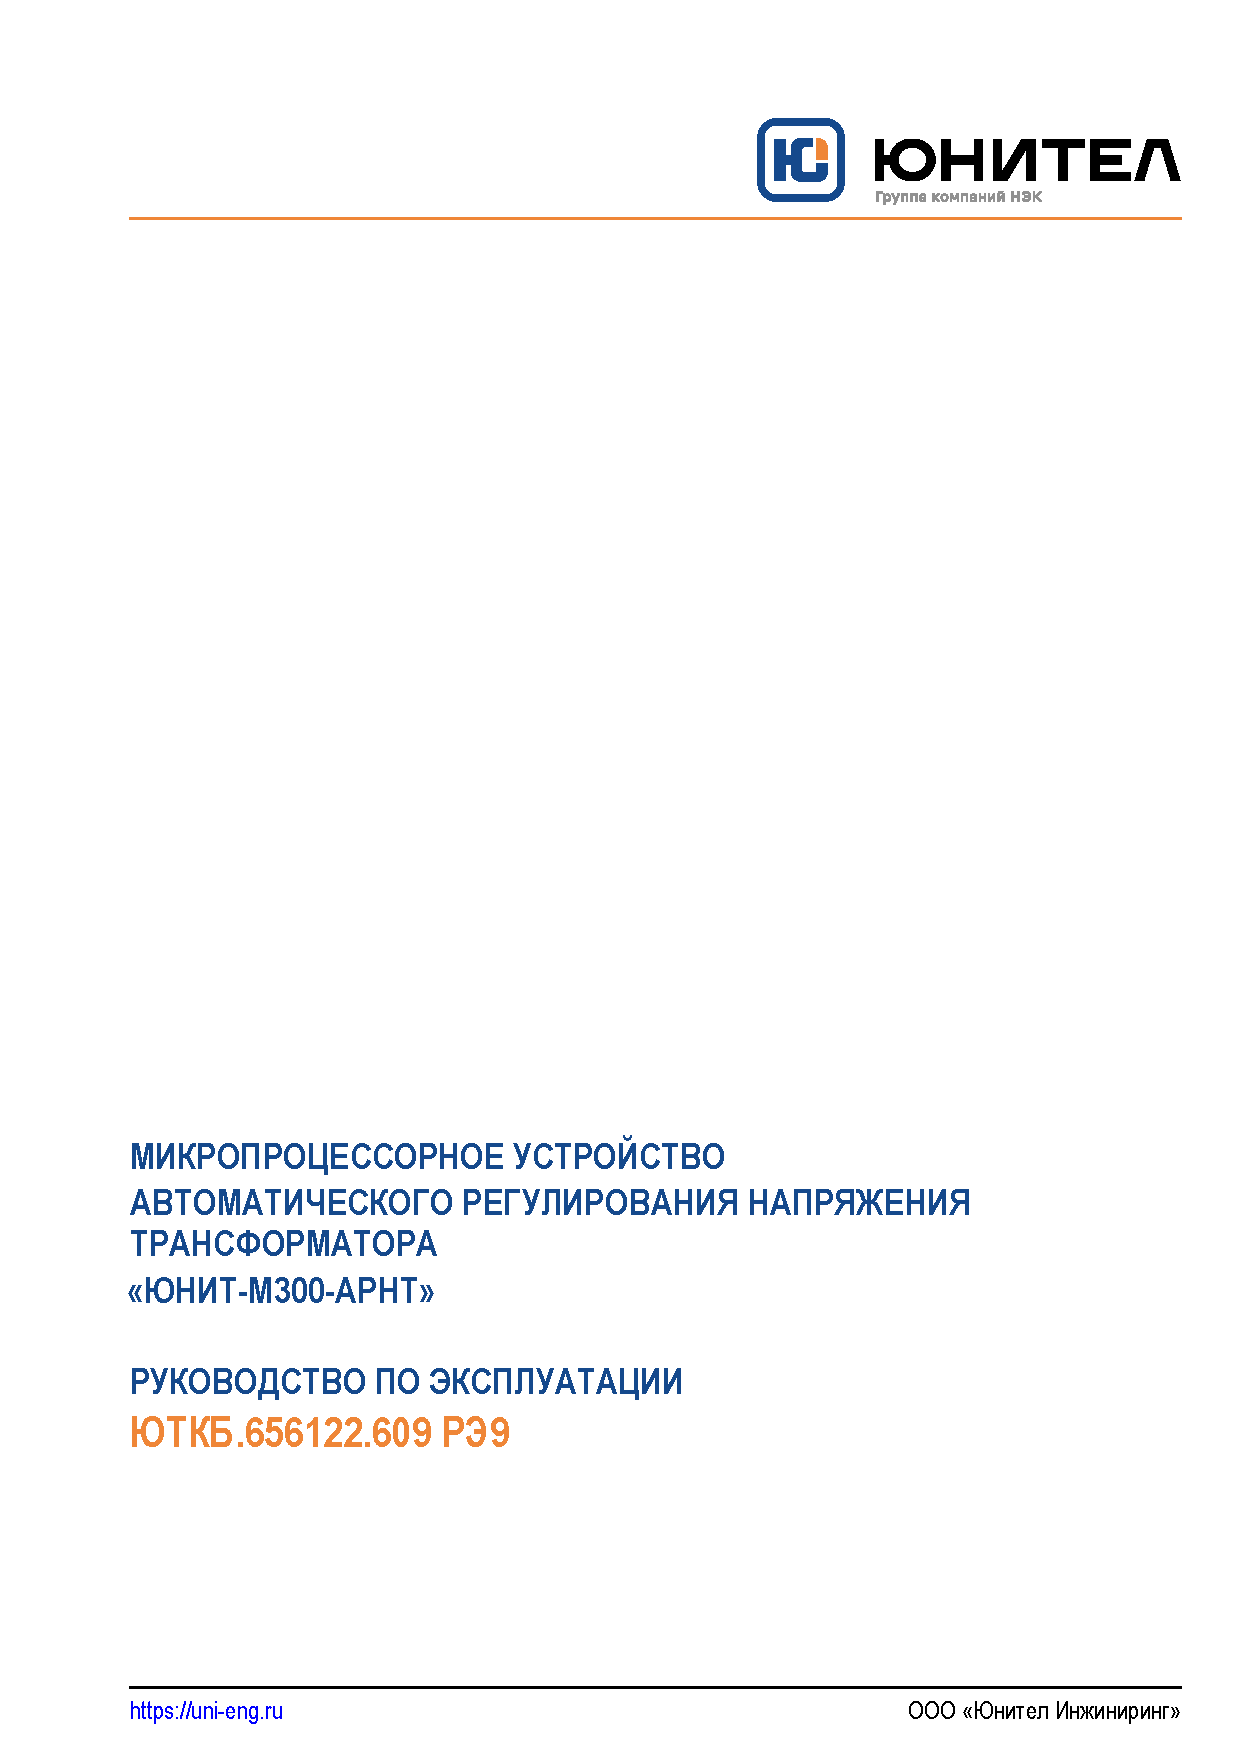
\includepdf[pages={1},width=0.5\textwidth, angle=90]{1.pdf} вставляем и поворачиваем pdf
%\begin{center}
%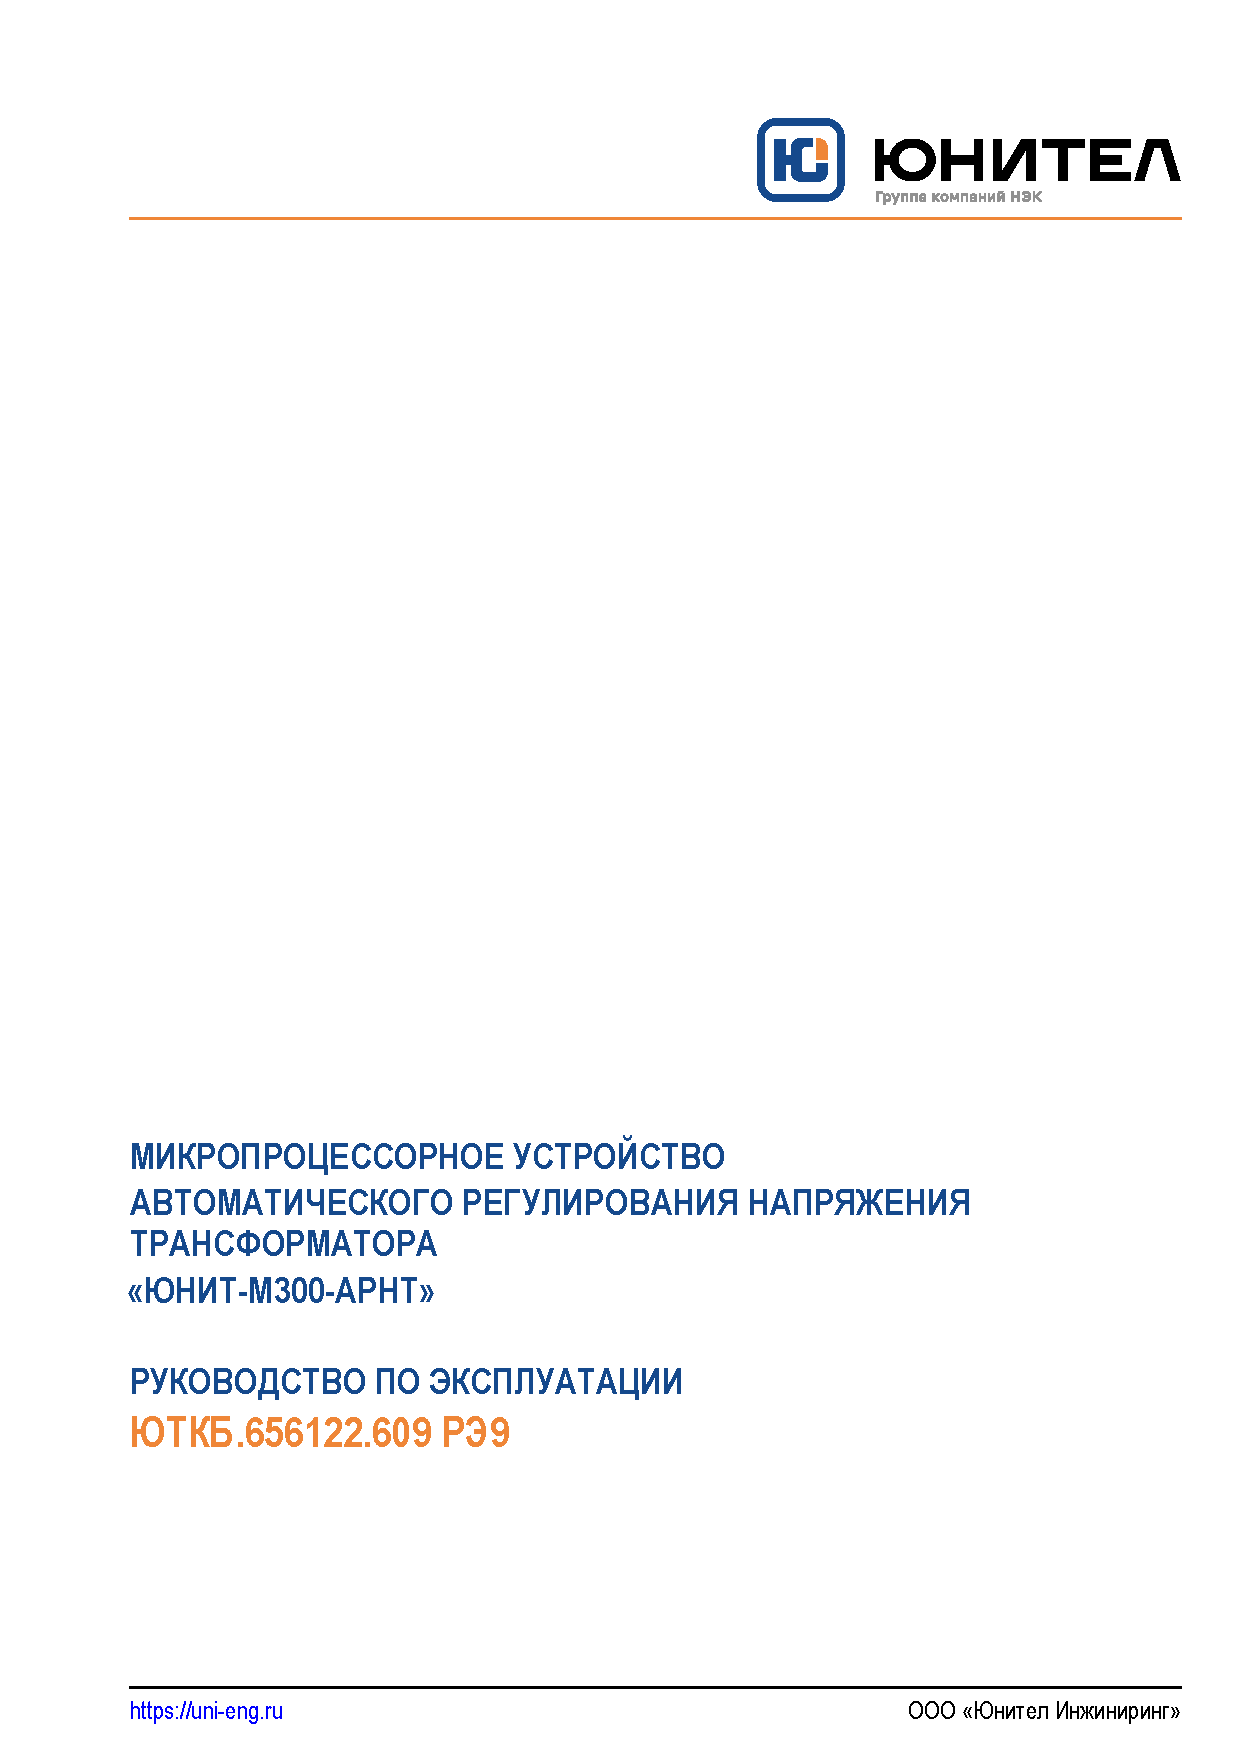
\includegraphics[width=1.4\textwidth]{1.pdf}
%\end{center}

\end{landscape}
\restoregeometry


